%%%%%%%%%%%%%%%%%%%%%%%%%%%%%%%%%%%%%%%%%
% Plain Cover Letter
% LaTeX Template
% Version 1.0 (28/5/13)
%
% This template has been downloaded from:
% http://www.LaTeXTemplates.com
%
% Original author:
% Rensselaer Polytechnic Institute 
% http://www.rpi.edu/dept/arc/training/latex/resumes/
%
% License:
% CC BY-NC-SA 3.0 (http://creativecommons.org/licenses/by-nc-sa/3.0/)
%
%%%%%%%%%%%%%%%%%%%%%%%%%%%%%%%%%%%%%%%%%

%----------------------------------------------------------------------------------------
%	PACKAGES AND OTHER DOCUMENT CONFIGURATIONS
%----------------------------------------------------------------------------------------

\documentclass[11pt]{letter} % Default font size of the document, change to 10pt to fit more text

\usepackage{newcent} % Default font is the New Century Schoolbook PostScript font
\usepackage{pdfpages}
%\usepackage{helvet} % Uncomment this (while commenting the above line) to use the Helvetica font

% Margins
\topmargin=-1in % Moves the top of the document 1 inch above the default
\textheight=8.5in % Total height of the text on the page before text goes on to the next page, this can be increased in a longer letter
\oddsidemargin=-10pt % Position of the left margin, can be negative or positive if you want more or less room
\textwidth=6.5in % Total width of the text, increase this if the left margin was decreased and vice-versa

\let\raggedleft\raggedright % Pushes the date (at the top) to the left, comment this line to have the date on the right

\begin{document}

%----------------------------------------------------------------------------------------
%	ADDRESSEE SECTION
%----------------------------------------------------------------------------------------

\begin{letter}{Mrs. Jane Smith \\
Recruitment Officer \\
The Corporation \\
123 Pleasant Lane \\
City, State 12345} 

%----------------------------------------------------------------------------------------
%	YOUR NAME & ADDRESS SECTION
%----------------------------------------------------------------------------------------

\begin{center}
\large\bf Daman Morris \\ % Your name
%\vspace{20pt} \hrule height 1pt % If you would like a horizontal line separating the name from the address, uncomment the line to the left of this text
1085 Nathaniel Rochester Hall \\ Rochester, NY 14623 \\ +1 (412) 586-8168 % Your address and phone number
\end{center}
\vfill

\signature{Daman Morris} % Your name for the signature at the bottom

%----------------------------------------------------------------------------------------
%	LETTER CONTENT SECTION
%----------------------------------------------------------------------------------------

\opening{To whom it may concern,}

I am writing this letter to apply for one of your open Software Engineering
Intern positions. I learned of this position through my school's career service
center and believe that my skillset could uniquely benefit the Corporation.

I have always been fascinated by computers and their workings, which led me to
develop a broad range of proficiency in a variety of software engineering
disciplines. My time at the Rochester Institute of Technology has helped me to
deepen this proficiency which will in turn, I hope, allow me to apply this
skillset to the benefit of the Corporation in any and all of its software
engineering needs. I have always strived to be as general-purpose as possible,
adapting best to whatever situation I find myself in, and so I believe that I
could excel at many of the Corporation's software development areas. My
attached résumé details my existing skills, but these can be extended and I
strive to do so constantly.

If possible, I would like to set up a personal interview so that my suitability
to both the position of Software Engineer and to the Corporation at large can
be better judged. I can be contacted at my personal phone number,
+1 (412) 586-8168, whenever is suitable. See also my attached résumé for
additional contact details. Thank you for taking the time to consider this
application, and I look forward to hearing from you.

\closing{Sincerely yours,}


%\encl{Curriculum vitae, employment form} % List your enclosed documents here, comment this out to get rid of the "encl:"

%----------------------------------------------------------------------------------------

\end{letter}

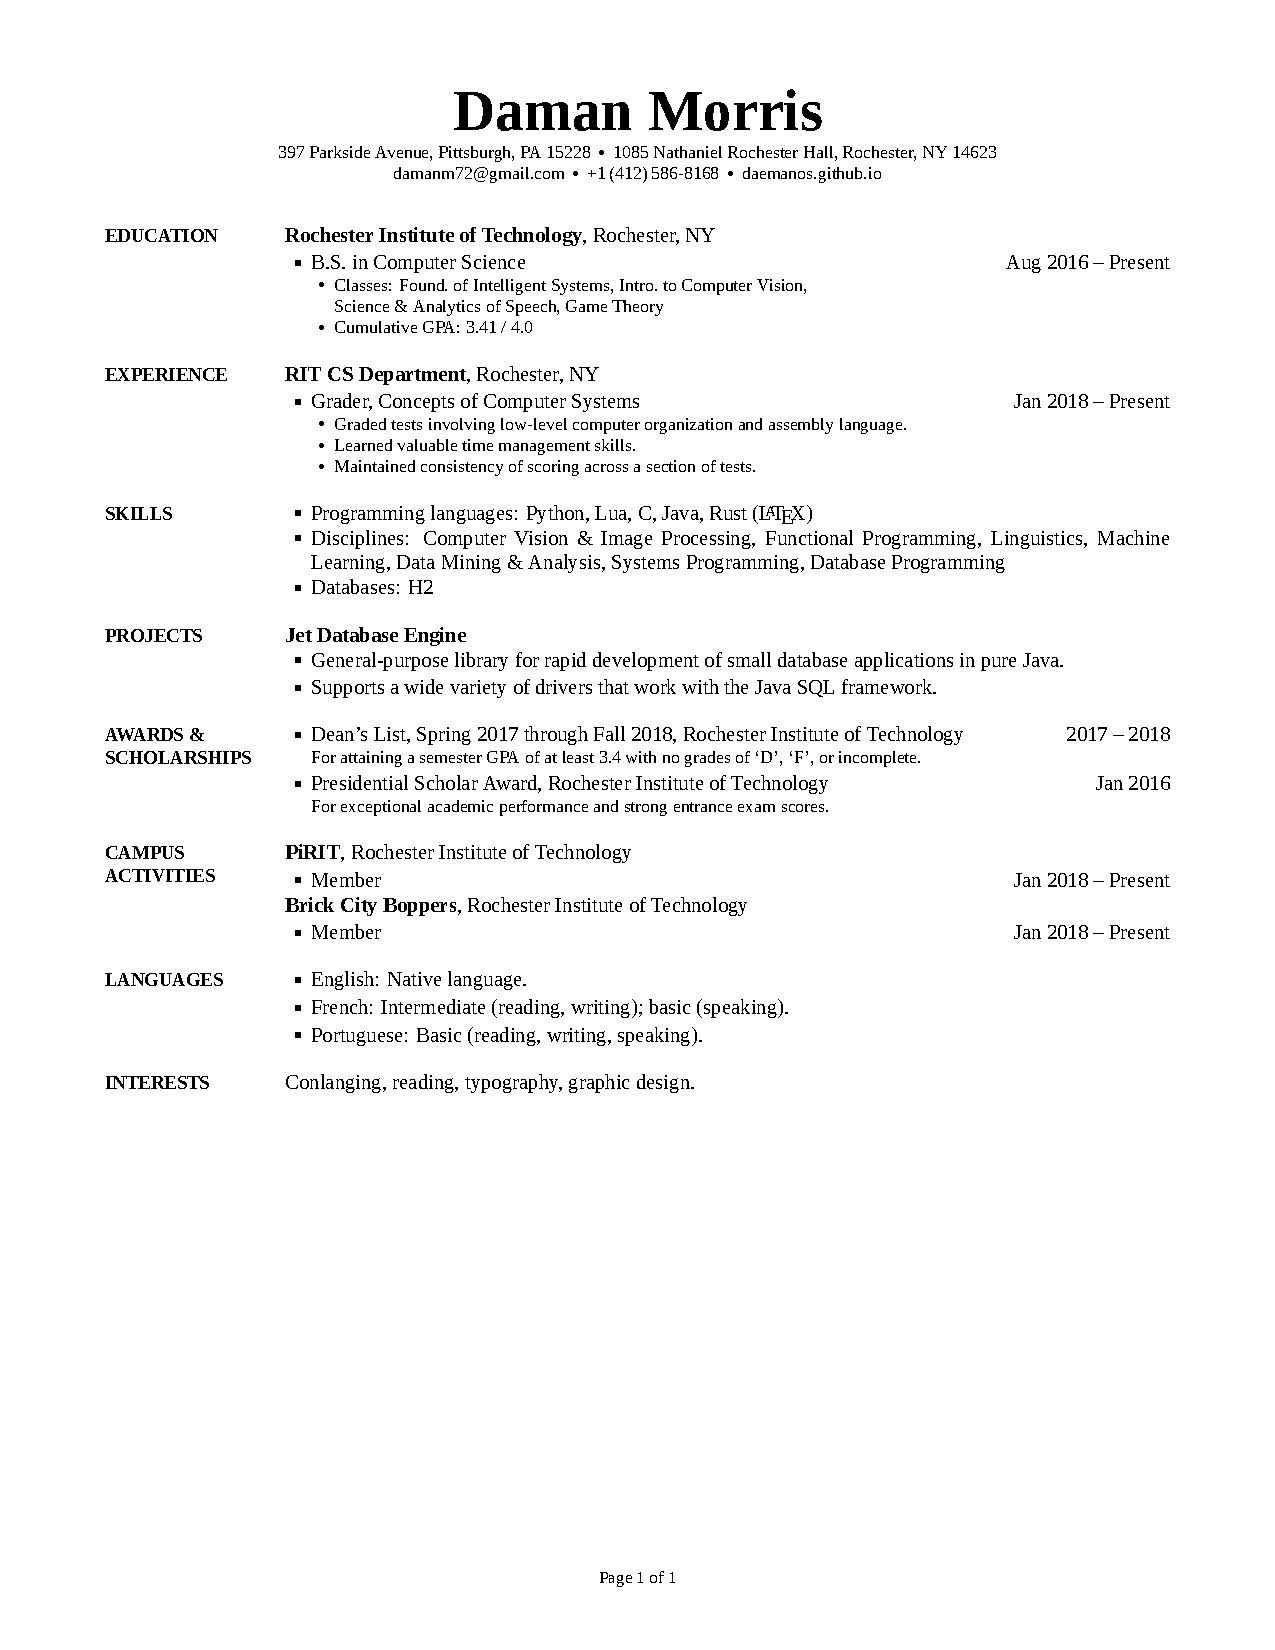
\includepdf{CV.pdf}

\end{document}
